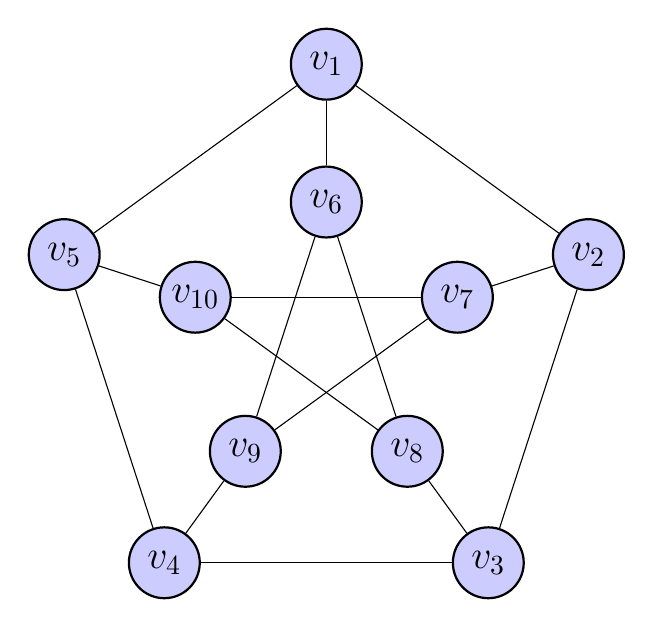
\begin{tikzpicture}[
  scale=1,
  vnode/.style={circle, fill=blue!20, draw=black, thick, minimum size=9mm, inner sep=0pt, font=\Large}
]
  % Vértices del pentágono exterior (en sentido horario desde arriba)
  \node[vnode] (v1) at (90:3.5)  {$v_1$};
  \node[vnode] (v2) at (18:3.5)  {$v_2$};
  \node[vnode] (v3) at (-54:3.5) {$v_3$};
  \node[vnode] (v4) at (-126:3.5) {$v_4$};
  \node[vnode] (v5) at (162:3.5) {$v_5$};

  % Vértices de la estrella interior (en sentido horario desde arriba)
  \node[vnode] (v6)  at (90:1.75)  {$v_6$};
  \node[vnode] (v7)  at (18:1.75)  {$v_7$};
  \node[vnode] (v8)  at (-54:1.75) {$v_8$};
  \node[vnode] (v9)  at (-126:1.75) {$v_9$};
  \node[vnode] (v10) at (162:1.75) {$v_{10}$};

  % Aristas
  \foreach \from/\to in {v1/v2, v2/v3, v3/v4, v4/v5, v5/v1,
                         v1/v6, v2/v7, v3/v8, v4/v9, v5/v10,
                         v6/v8, v8/v10, v10/v7, v7/v9, v9/v6}
    \draw (\from) -- (\to);
\end{tikzpicture}
